
% Due Date: 6/11/14

\chapter{The Legion Programming Model}
\label{chapter:model}
In this chapter we outline the design of the
Legion programming model.  We describe the
important features of Legion as well as 
their interactions to create a composable programming
infrastructure. We emphasize that the Legion
programming model is general enough to be 
implemented in most modern programming languages
and is not tied to any particular language.
In this chapter we focus solely on the features
of the programming model and do not describe
how they are implemented.  Our discussion of
the implementation of the Legion runtime begins
in Chapter~\ref{chapter:arch}. We start with 
a motivating example to illustrate some of the
features of Legion, and how they address many
of the problems encountered when writing code
for distributed heterogeneous architectures.


\section{Motivating Example: Circuit Simulation}
\label{sec:circuit}
To make our introduction of the features of
Legion concrete, we use a circuit simulation as
a running example. Listing~\ref{lst:code_ex}
shows pseudo-code for an electrical circuit simulation
written in a C-like language. The circuit simulation
represents the circuit as a graph consisting of nodes
with different voltage and edges representing various
circuit components. At each time step the simulation 
calculates currents, distributes charge between different 
nodes, and updates the voltage at each node. We provide 
a brief overview of the code here. The details of the 
pertinent Legion abstractions are covered in the 
following sections.

\lstset{
  captionpos=b,
  language=C++,
  basicstyle=\scriptsize,
  numbers=left,
  numberstyle=\tiny,
  columns=fullflexible,
  stepnumber=1,
  escapechar=\#,
  keepspaces=true,
  literate={<}{{$\langle$}}1 {>}{{$\rangle$}}1,
  morekeywords={region,coloring,partition,disjoint,aliased,tunable,future,predicate,spawn},
  deletekeywords=float,
}
\begin{lstlisting}[float,floatplacement=H,label={lst:code_ex},caption={Circuit simulation}]
struct Node { float voltage, new_charge, capacitance; };
struct Wire<rn> { Node@rn in_node, out_node; float current, ... ; };
struct Circuit { region   r_all_nodes; /* contains all nodes for the circuit */
                 region   r_all_wires; /* contains all circuit wires */ };
struct CircuitPiece {
  region  rn_pvt, rn_shr, rn_ghost; /* private, shared, ghost node regions */
  region  rw_pvt;                   /* private wires region */ };

void simulate_circuit(Circuit c, float dt) : RWE(c.r_all_nodes, c.r_all_wires)
{
  // The construction of the colorings is not shown.  The colorings wire_owner_map,
  tunable int num_pieces;
  // node_owner_map, and node_neighbor_map have num_pieces _PIECES colors 
  // 0..num_pieces #$-$# 1. The coloring node_sharing map has two colors 0 and 1.
  //
  // Partition of wires into num_pieces pieces
  partition<disjoint> p_wires = c.r_all_wires.partition(wire_owner_map); 
  // Partition nodes into two parts for all-private vs. all-shared
  partition<disjoint> p_nodes_pvs = c.r_all_nodes.partition(node_sharing map);

  // Partition all-private into num_pieces disjoint circuit pieces
  partition<disjoint> p_pvt_nodes = p_nodes_pvs[0].partition(node_owner_map);
  // Partition all-shared into num_pieces disjoint circuit pieces
  partition<disjoint> p_shr_nodes = p_nodes_pvs[1].partition(node_owner_map);
  // Partition all-shared into num_pieces ghost regions, which may be aliased
  partition<aliased> p_ghost_nodes = p_nodes_pvs[1].partition(node_neighbor_map);

  CircuitPiece pieces[num_pieces];
  for(i = 0; i #$<$# num_pieces; i++) 
    pieces[i] = { rn_pvt: p_pvt_nodes[i], rn_shr: p_shr_nodes[i],
                  rn_ghost: p_ghost_nodes[i], rw_pvt: p_wires[i] };
  for (t = 0; t #$<$# TIME_STEPS; t++) {
    for (i = 0; i #$<$# num_pieces; i++) calc_new_currents(pieces[i]);
    for (i = 0; i #$<$# num_pieces; i++) distribute_charge(pieces[i], dt);
    for (i = 0; i #$<$# num_pieces; i++) update_voltages(pieces[i]);
  }
}
                           // ROE = Read-Only-Exclusive
void calc_new_currents(CircuitPiece piece):
        RWE(piece.rw_pvt), ROE(piece.rn_pvt, piece.rn_shr, piece.rn_ghost) {
  foreach(w : piece.rw_pvt)
    w#$\rightarrow$#current = (w#$\rightarrow$#in_node#$\rightarrow$#voltage - w#$\rightarrow$#out_node#$\rightarrow$#voltage) / w#$\rightarrow$#resistance;
}
                          // RdA = Reduce-Atomic
void distribute_charge(CircuitPiece piece, float dt):
        ROE(piece.rw_pvt), RdA(piece.rn_pvt, piece.rn_shr, piece.rn_ghost) {
  foreach(w : piece.rw_pvt) {
    w#$\rightarrow$#in_node#$\rightarrow$#new_charge += -dt * w#$\rightarrow$#current;
    w#$\rightarrow$#out_node#$\rightarrow$#new_charge +=  dt * w#$\rightarrow$#current;
  }
}

void update_voltages(CircuitPiece piece): RWE(piece.rn_pvt, piece.rn_shr) {
  foreach(n : piece.rn_pvt, piece.rn_shr) {
    n#$\rightarrow$#voltage += n#$\rightarrow$#new_charge / n#$\rightarrow$#capacitance;
    n#$\rightarrow$#new_charge = 0;
  }
}
\end{lstlisting}

\begin{figure}[t]
  \centering
\subfloat[Node region tree.]{
\label{sfig:part_fig:tree}
%\begin{tikzpicture}[scale=0.8]
%\partitiontree
%\end{tikzpicture}
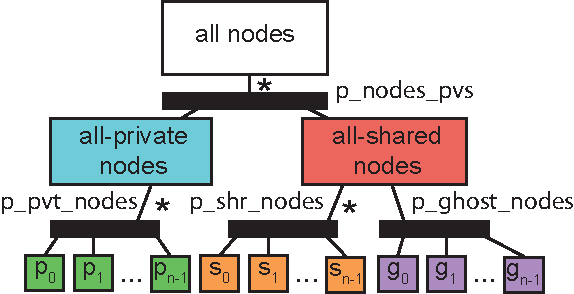
\includegraphics[scale=0.60]{figs/CircuitPartition.pdf}
}

  \subfloat[$p\_nodes\_pvs$]{
\label{sfig:part_fig:pvs}
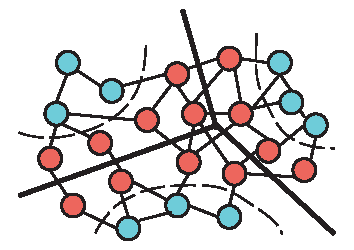
\includegraphics[scale=0.60]{figs/Private_vs_Shared.pdf}
}
  \subfloat[$p_i$]{
\label{sfig:part_fig:p_i}
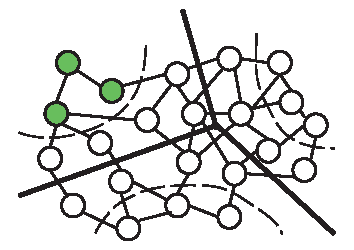
\includegraphics[scale=0.60]{figs/Private_Local.pdf}
}
  \subfloat[$s_i$]{
\label{sfig:part_fig:s_i}
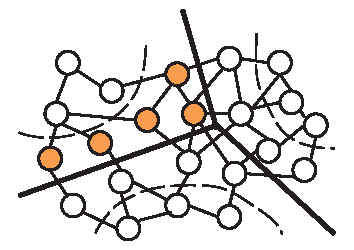
\includegraphics[scale=0.60]{figs/Shared_Local.pdf}
}
  \subfloat[$g_i$]{
\label{sfig:part_fig:g_i}
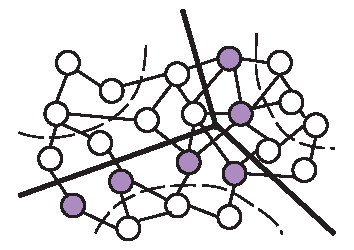
\includegraphics[scale=0.60]{figs/Ghost_Local.pdf}
}
  \caption{Partitions of $r{\_}all{\_}nodes$\label{fig:part_fig}}
\end{figure}

A {\tt Circuit} structure contains handles to the
names of two logical regions: a collection of nodes 
and a collection of wires (lines 3-4 of 
Listing~\ref{lst:code_ex}).\footnote{Note that all 
pointers declare the region to which they point.  For
example, the definition of {\tt Wire} (line 2) is 
parametrized on the region {\tt rn} to which the 
{\tt Node} pointers in fields {\tt in\_nodes}
and {\tt out\_nodes} point.} It is important to note
that logical regions simply describe collections of data
and do not imply any placement or layout in the
memory hierarchy. We discuss how logical regions are
created and used starting in Section~\ref{sec:logicalreg}.

\subsection{Circuit Regions and Partitions}
\label{subsec:circuitregpart}
In order to run the circuit simulation in parallel, 
the circuit graph must be partitioned into {\em pieces}
that can be distributed throughout the memory hierarchy.
The number of pieces to create is ultimately chosen
by the mapper based on application and architecture
specific considerations; the mapper's decision is
communicated by a {\em tunable} variable\cite{Sequoia06}.
Tunable values are necessary for abiding by our second 
design principle of decoupling specification from mapping.
The choice of how many pieces to create is machine specific
and therefore must be determined as part of the mapping
process.

Traditionally, a graph, such as the one for our circuit
simulation, is only partitioned a single time into 
different pieces based on the number of nodes
for the target machine. This single partitioning scheme,
however, fails to capture all of the different relationships
between nodes and wires within the circuit graph. Instead,
our Legion circuit simulation employs a two-level
partitioning scheme to more precisely capture information
about the different sets of the circuit graph necessary
for implementing the circuit simulation.

Figure~\ref{sfig:part_fig:tree} depicts a {\em logical
region tree} data structure that demonstrates how
the nodes for the circuit graph can be better represented
using a multi-level partitioning into logical sub-regions. 
Intuitively, the logical region tree data structure
shows how the nodes within the graph our broken down
into subsets represented by logical sub-regions.
Our multi-level partitioning is still based on the 
idea of creating circuit pieces, but we describe the
pieces as a union of different subsets. We first partition
all the nodes into two distinct subsets, the 
{\em all-private} and {\em all-shared} nodes. These 
different sets are depicted in Figure~\ref{sfig:part_fig:pvs}.
The all-private nodes are colored in blue (light-grey)
and have no edges which cross a piece boundary. The
all-shared nodes are colored in red (dark-grey), and
have at least one edge that crosses a piece boundary.
This {\em coloring} of the nodes is reflected in the
code by the {\tt node\_sharing\_map} (line 19) that
is passed to Legion to create a partition of the 
logical region containing all nodes. The resulting 
partition {\tt p\_nodes\_pvs} has exactly two logical
sub-regions (one for each color), with each node
belonging to the logical sub-region based on how it
was colored. We discuss the details of partitioning
further in Section~\ref{sec:partitioning}.

After our first level of partitioning, we again
partition the two logical sub-regions for the all-private
and all-shared sub-regions again to describe the
subsets for different circuit pieces. Lines 22 and 24
show the calls to partition each of these two sub-regions
into further sub-regions describing the subsets for
different circuit pieces. The coloring for the upper-left
circuit piece for the private and shared nodes is
shown in Figures~\ref{sfig:part_fig:p_i} and 
\ref{sfig:part_fig:s_i} respectively. 

Another feature of the Legion programming model is 
that it allows multiple partitions of logical regions 
to be made, creating multiple views onto the same set 
of data. For example, in the circuit simulation, we also 
need to create an additional partition for describing 
the {\em ghost nodes} necessary for each circuit piece. 
Figure~\ref{sfig:part_fig:g_i} shows the coloring for 
the ghost nodes of the piece in the upper left of the 
circuit graph. The ghost node partition is a second 
partition of the all-shared logical region. Note that
unlike prior partitions, the ghost node partitioning
may color some nodes with multiple colors because
some nodes share edges with multiple pieces. We therefore
say that this is an {\em aliased} partition since not all
of the sub-regions are disjoint (line 26). The ability
of the Legion programming model to capture disjointness
and aliasing properties of logical regions will be
crucial for constructing a high-performance implementation
of Legion.

Based on the logical sub-regions that we create, we
can now create circuit pieces for different
logical sub-regions. Lines 5-7 of 
Listing~\ref{lst:code_ex} declare the type of
a {\tt CircuitPiece} structure. Each circuit piece is
defined by the private, shared, and ghost logical
sub-regions in the logical region tree of all nodes.
A circuit piece also names the set of wires that it
uses. There is a single disjoint partitioning of the
wires logical region into sub-regions based on pieces
on line 17. Lines 29-31 then assemble the different
circuit pieces for our simulation. It is important
to note that the entire assembly of the circuit pieces
is done dynamically, including the coloring and 
partitioning operations. The dynamic nature of this
process allows Legion to adapt to both the circuit
topology as well as the underlying machine structure
at runtime.

A final important detail regarding the partitioning
for the circuit simulation is that the actual choice
of the partitioning into pieces was selected by
the application and not Legion. This reflects our
first design principle that we should decouple policy
from mechanism. It is the responsibility of the 
application to choose the partitioning algorithm (policy)
for creating the pieces.  Legion then provides the 
mechanism for capturing the result: specifically the
colorings for creating partitions and logical sub-regions.
Regardless of the chosen partitioning algorithm, 
colorings are flexible enough to capture the resulting
partitioning.

\subsection{Circuit Tasks and Operations}
\label{subsec:circuittasks}
Line 9 of Listing~\ref{lst:code_ex} declares 
the main function for the circuit simulation.
The {\tt simulate\_circuit} function is an example 
of a Legion task. All Legion tasks are required to
name the logical regions they access along with
the {\em privileges} and {\em coherence modes}
with which they access the logical regions. The
privilege and coherence annotation {\tt RWE} on
line 9 specifies that the {\tt simulate\_circuit}
task will access the logical regions {\tt c.r\_all\_nodes}
and {\tt c.r\_all\_wires} with {\em read-write} 
privileges and {\em exclusive} coherence. Privileges
specify the kind of side-effects the task can perform
on the logical region. Coherence specifies what
other tasks can do with regions at the same time
as the task using the regions (if anything). We
discuss tasks and privileges in more detail in 
Section~\ref{sec:tasks}. Coherence modes are part
of an extension to the Legion programming model
that we cover in Chapter~\ref{chapter:relaxed}.

Lines 32-58 perform the actual circuit simulation 
by making three passes over the circuit for each 
time step.  Each pass loops over the array of 
pieces (constructed on lines 29-31 from the 
partitions) and asynchronously launches a sub-task 
computation to be performed for each piece. There 
are  no explicit requests for parallel execution 
in Legion nor is there 
explicit synchronization between the passes.  
Which tasks can be run in parallel within a 
pass and the required inter-pass dependencies are
determined automatically by the Legion runtime 
based on the region access annotations on the 
task declarations. The details of how these
dependences are covered can be found in our
description of the Legion execution model
in Section~\ref{subsec:execmodel}.

The tasks launched on lines 33-35 are 
{\em sub-tasks} of the main {\tt simulate\_circuit} 
task. A sub-task can only access regions (or 
sub-regions) that its parent task could access; 
furthermore, the sub-task can only have permissions 
on a region compatible with the parent's permissions. 
For example, the {\tt calc\_new\_currents} task reads 
and writes the wires sub-region and reads 
the private, shared, and ghost node sub-regions 
for its piece (line 40). The requested regions for the 
{\tt calc\_new\_currents} task therefore meet
the requirements of the Legion programming model.
We discuss the additional types of privileges available
for tasks to use in Section~\ref{subsec:privileges}.

The implementation of each of the different {\em leaf}
tasks for our simulation are shown on lines 39-58.
Leaf tasks are tasks that perform only computation
and do not perform any additional Legion operations.
In general, tasks are permitted to recursively launch
additional sub-tasks which we discuss in 
Section~\ref{subsec:subtasks}. Tasks are also permitted
to perform other kinds of operations such as inline
mapping, explicit copies, and execution fences that
are discussed in Section~\ref{sec:ops}.

%The {\tt distribute\_charge} 
%task reads the piece's wires subregion and 
%updates all nodes those wires touch.  

%However,
%rather than using read/write privilege for the 
%nodes (which would serialize these tasks for 
%correctness), the task uses reorderable 
%reduction operations and atomic rather than 
%exclusive access. The final task 
%{\tt update\_voltages} writes the shared 
%and private nodes for a piece and reads the 
%results of the previous task's reductions.


\section{Logical Regions}
\label{sec:logicalreg}
The primary abstraction for describing data in
Legion is {\em logical regions}. The motivation for 
logical regions stems directly from our second design
principle regarding decoupling application specification
from mechanism. While many programming systems have
abstractions for computation, few systems have data
models for abstracting the description of program data.
Logical regions decouple the 
description of data from any mapping related data decisions:

\begin{itemize}
\item Logical regions have no implied location or
      placement in the memory hierarchy.
\item Logical regions have no implied layout of
      data in memory such as struct-of-arrays (SOA), 
      array-of-structs (AOS), hybrid, etc.
\end{itemize}

As an example, recall from the circuit simulation in 
Section~\ref{sec:circuit} how logical regions capture the 
structure of the circuit graph and the various important
subsets without committing to the placement or layout
of any data. Logical regions, therefore, provide the 
crucial abstraction for describing the structure of 
program data without constraining data to any 
particular target architecture, thus taking the first 
step in decoupling the specification of an application 
from its mapping. We now detail how logical regions
are created and used.

\subsection{Relational Data Model}
\label{subsec:relations}
To describe the structure of program
data, we require that logical regions be 
general enough to support arbitrary data structures.
To meet this need, we drew inspiration from databases
and the work in \cite{Hawkins11} that demonstrated
that {\em relations} are a general abstraction capable
of encoding most complex data structures in use in
real applications. For example, in the circuit simulation,
the graph of circuit elements is easy to encode as two
separate relations: one for describing the 
sets of nodes, and another for describing the 
sets of wires. Logical regions are therefore
based on relations and have notions of {\em index
spaces} (e.g. sets of rows) and {\em field spaces}
(e.g. columns).  We describe each of these properties
in detail in Sections~\ref{subsec:indexspace} and
\ref{subsec:fieldspace} respectively.

Before proceeding, it is important to note that logical
regions in many ways are not full relations in the
traditional database sense. Relations in databases
normally support a full (or nearly full) implementation
of relational algebra including operations such as inner 
and outer joins. In Legion, our goal is not to re-implement
a database system. Instead, we are adapting the
relational data model provided by relations to
serve as the basis for describing data in Legion
programs, and supporting a minimal subset of relational
algebra necessary for describing the operations
used to achieve high performance on our target class of
machines. We highlight the important Legion operations
that have natural analogs to database operations where
appropriate.

\subsection{Index Spaces}
\label{subsec:indexspace}
To describe the rows of logical regions we use
{\em index spaces}.  Index spaces encapsulate
the keys for logical regions. Currently, Legion
permits two different kinds of index spaces
to be created for describing the sets of
keys: {\em unstructured} and {\em structured}
index spaces. By specifying different kinds of
index spaces, applications can indicate the best
representation for index spaces. Unstructured
index spaces suggest that there is little
structure in the keys, while structured index
spaces are used for representing index spaces
with one or more collections of dense keys
(e.g. N-dimensional Cartesian grids). We now
describe each of these kinds of index spaces
in turn.

Unstructured index spaces capture arbitrary
collections of keys and allow
for the dynamic allocation and freeing of 
opaque keys that we call {\em pointers}. Note
that these pointers are significantly different
from traditional pointers in a language such as
C. Pointers in C imply a specific location in
memory where data has been allocated. In Legion,
pointers are simply keys for accessing logical
regions associated with a given index space.
Thus pointers in Legion are portable and can
be used regardless of where a logical region
has been mapped. One similarity with C pointers
is that Legion permits dynamic allocation and the freeing 
of pointers in an unstructured index space, much
like how C permits dynamic memory allocation
and freeing. The logical regions in our 
circuit simulation use unstructured index spaces
due to the irregular nature of the graph. Both
the logical region containing node data and the
logical region containing wire data are based on 
unstructured index spaces and pointers are allocated 
in these index spaces as necessary based on 
the topology of the graph.

In contrast to unstructured index spaces, structured
index spaces are represented by one or more 
Cartesian grids of points. If more than one grid
is specified, they must all be of the same dimension.
We use these kinds of index spaces for describing
applications with more regular structures such
as linear algebra and applications that work on
regular grids like S3D (see Chapter~\ref{chapter:s3d}).

The Legion programming model is also open to extension
in the variety of kinds of index spaces.  Presently, 
only two kinds of index spaces are supported; however, we envision 
having many different kinds of index spaces for 
representing different sparsity patterns. For example,
in the case of sparse matrix applications, it
is useful to represent different sparse matrices
in different ways based on the local structures
they contain within them. For these cases we want
Legion to be able to support index spaces that
capture different ways of efficiently representing
keys for different entries in a logical region.

It is important to note that our design of index
spaces strictly adheres to our first design principle
of separating policy from mechanism. Legion
applications can completely control the
kind of index spaces when creating logical regions,
thereby specifying the policy to use for different
kinds of data. Independently, the mechanisms for
implementing each of the various kinds of index
space are completely contained within the Legion 
runtime and opaque to the programmer, thereby
allowing Legion to manage the complexity of the
implementation and to incorporate optimizations
for specific target architectures.

\subsection{Field Spaces}
\label{subsec:fieldspace}
To represent the columns (also called fields) of 
logical regions, Legion uses {\em field spaces}. 
Field spaces encapsulate the set of all fields
available in a logical region. Each field is
defined by a pair of values: a unique name
for the field (usually an integer), and the
type of the field.  The type of a field can 
be either a plain old data (POD) type (in the 
traditional C sense), or a compound type. Legion 
users are free to decide the whether fields should 
consist of POD base types or compound types with
the understanding that the finest granularity at
which Legion will be able to reason about data
is at the granularity of individual fields. 

Field spaces are another example of the decoupling
of policy and mechanism in Legion. Field spaces
allow users to control the policy of what
constitutes a field in a field space, while
Legion provides the mechanisms for how field
spaces are implemented and used.  For our circuit 
simulation each POD type associated with either a node
or a wire (e.g. charge, voltage, capacitance, etc.)
is made into an individual field in a field space, 
thus giving Legion total visibility of all the fields 
within both the node and wire logical regions.

One important restriction of field spaces in
Legion is that we require that the maximum number
of fields in a field space be statically upper
bounded. This restriction is necessary for an
efficient Legion implementation, described 
in more detail in Section~\ref{subsec:fieldmasks}.
It is important to note that this restriction does
not limit the expressivity of Legion as applications
are free to create an unlimited number of field spaces
(and corresponding logical regions) and therefore the
total number of fields in any application is unbounded.
The restriction only places a cap on the maximum number
of fields in a single field space.

\subsection{Region Trees}
\label{subsec:trees}
Logical regions in Legion are created by taking
the cross product of a field space with an index
space. Each invocation of this cross product generates 
a new logical region. Logical regions created in 
this way can also be partitioned into logical sub-regions
that we discuss in Section~\ref{sec:partitioning}. We refer 
to a logical region and all of its logical sub-regions as 
a {\em region tree}. Since each cross-product of a
field space with an index space results in a new
logical region, we assign to each region tree a 
{\em tree ID}. Therefore, each logical region can be
uniquely identified by a 3-tuple consisting of 
an index space, a field space, and a tree ID. An
alternative design would have been to define
each cross-product of a field space with an 
index space as a unique logical region. Ultimately, we
decided that it is beneficial in many cases
to define multiple logical regions based on the
same field space and index space. We will give an
example of this pattern in Chapter~\ref{chapter:s3d}.

The dynamic nature of logical regions is important.
Field spaces, index spaces, and logical regions can
all be created and destroyed at runtime.  This gives 
applications the freedom to dynamically determine
both the number and properties of logical regions.
By making all operations associated with index spaces,
field spaces, and logical regions dynamic, Legion is well
positioned to react to the dynamism in both software
and hardware described in Section~\ref{subsec:dynamism}.

\section{Partitioning}
\label{sec:partitioning}
When writing code for distributed memory architectures,
one of the most important components of an application
is determining how data is partitioned. Traditionally, 
partitioning of data is done to assign different subsets 
of data to different nodes. In Legion, partitioning 
is designed to be a more general operation, not tied to 
an actual distribution of data to specific nodes. Instead, 
partitioning in Legion is an operation that is used
to name different subsets of data that will be
used by different computations. Drawing an analogy
to relational database systems, logical sub-regions
are similar to views onto a subset of a relation.
Furthermore, Legion supports hierarchical partitioning,
allowing subsets to be further refined, in order to 
describe tiered sets of data. By creating hierarchical 
logical sub-regions through partitioning, applications 
can precisely scope the set of data used 
by different computations.

In keeping with our first design principle, Legion
does not provide any automated partitioning schemes.  
Instead it is the responsibility of the application 
to determine the best way to partition data for the 
computation it intends to perform, thereby specifying 
the policy for how to partition data.  In conjunction,
Legion provides the mechanism for capturing the result
of the partition in terms of logical regions. For example,
in the circuit simulation, the partitioning of the circuit
graph into pieces could be done by a third party library
such as METIS. The results of the computed partitioning are 
then captured by Legion in the form of partition objects
with logical sub-regions.

Creating partitions with logical sub-regions 
is done with {\em colorings}.  Colorings are objects
that describe an intended partition of an index space.
Technically, a coloring is a map from {\em colors} to sets of
points in an index space. For unstructured index spaces,
colorings are maps from colors to sets of individual pointers,
while for structured index spaces colorings are maps from
colors to one or more Cartesian groups of points. For each 
color in a coloring, Legion will create one logical index 
sub-space of the parent index space. For every logical 
region based on the parent index space, a corresponding 
logical sub-region will exist for the newly created index 
sub-space. Figure~\ref{fig:part_fig} illustrates this
process for the circuit simulation.

Partitions in Legion are normally used to create multiple
logical sub-regions simultaneously.  Legion records two
important properties about the set of logical sub-regions
created in a partition. First, Legion records whether the
index sub-spaces that are created by a partition are 
{\em disjoint}. A partitioning is defined to be disjoint if
each entry in the parent index space of the partition is
assigned to at most one of the index sub-spaces. Legion does
permit colorings in which a single point in the parent
index space is assigned to multiple index sub-spaces. 
Partitions containing points colored more than once are
called {\em aliased}, since some index sub-spaces
contain the same point\footnote{
More mathematically inclined readers may prefer to think
of colorings as a relation (in the mathematical sense), with
the relation being considered disjoint if it is a function,
and aliased otherwise.}.

The second property of partitions tracked by Legion is
{\em completeness}. If every point in a parent index space
is mapped to at least one of the index sub-spaces, then
the partition is said to be complete, otherwise it is
incomplete\footnote{For mathematically inclined readers,
this property is surjectivity.}. We will see how Legion
benefits from tracking these properties of partitions
in Chapters~\ref{chapter:logical} and \ref{chapter:physical}.

\subsection{Tunable Variables}
\label{subsec:tunablevars}
Another example of separating specification from mapping
in the design of Legion is {\em tunable
variables}. In many cases, partitioning is done based 
on the size of the machine and the number of processors 
available for different computations, all of which are 
aspects of the target machine. There obviously exists a 
natural tension with our second design goal that requires
algorithm specification to be decoupled from the mapping.
To handle this decoupling we borrow an idea from the
Sequoia programming model \cite{Sequoia06}, and provide
tunable variables as a feature of Legion.

Tunable variables are assigned a 
value at runtime by a Legion mapper. While we defer our 
discussion of Legion mapper objects until 
Chapter~\ref{chapter:mapping}, for now it is sufficient 
to know that Legion mappers can determine the value of 
tunables based on both machine and application specific 
information. By explicitly describing 
a variable as a tunable, applications can decouple the
specification of an application from its mapping,
ultimately allowing mappers to determine optimal values
for tunables. For example, in the circuit simulation, a
tunable variable is used to determine the number of
pieces to direct METIS to compute for the circuit
graph. The mapper that picks this value is likely
to make the determination of the tunable value based
on the number of nodes or number of processors in 
the target machine. For example, in our circuit
simulation we use the tunable variable {\tt num\_pieces}
(line 12 in Listing~\ref{lst:code_ex}) to determine
the number of pieces to create when partitioning
the circuit graph. The mapper will likely determine
the value for this tunable variable based on 
the number of nodes or processors in the machine.

There are two important details regarding tunable
variables.  First, tunable variables are not specific
to partitioning, and can be used for any purpose in
any task. This allows applications to explicitly declare
any variable that should be explicitly chosen by
a mapper as a tunable variable. Second, unlike the 
statically-specified tunable variables in Sequoia,
tunable variables in Legion are dynamically determined. 
This allows mappers to change the values that it assigns to
tunable variables across different task instances
and react to changes in the hardware or software
as part of assigning specific values to tunable variables.

\subsection{Multiple Partitions}
\label{subsec:multiple}
One of the most important aspects of the Legion
programming model is that it supports multiple
partitions of an index space.  Multiple partitions
allow applications to describe many different
views onto the same collection of data. Supporting
multiple partitions is
important because most data in applications is
viewed in different ways depending on the phase
of the computation. For example, in the circuit 
simulation, there are shared nodes that have at
least one edge that crosses a piece boundary.  In
some cases, these shared nodes need to be accessed
by computations on the piece that owns them, while
in other cases, shared nodes are accessed as 
ghost nodes for an adjacent piece. Being able to
capture these multiple views onto the same data
is crucial to capturing the data usage patterns
of real applications.

\subsection{Recursive Partitions}
\label{subsec:recursivepart}
Another important aspect of Legion is that it
supports recursive partitions. Applications can
recursively partition index sub-spaces into further
index sub-spaces, thus creating arbitrarily deep
index trees and corresponding logical region trees.

The ability to create recursive partitions is 
important for two reasons. First, recursive partitions
allow applications to partition data in a way that
aligns with deep memory hierarchies, which was
one of the key insights of the Sequoia programming
language \cite{Sequoia06}. Second, supporting 
recursive partitioning is necessary for capturing
non-trivial subsets of data. For example, the circuit
simulation uses two levels of partitioning to first
break nodes into all-private and all-shared nodes, and 
then recursively partitions those sub-regions to express
the subsets of nodes in each of the pieces. This 
allows the logical region tree to capture important
disjointness information about the different subsets
of nodes.

\subsection{Interaction with Allocation}
\label{subsec:partalloc}
Partitioning in Legion is flexible enough to support
two different approaches that we term
{\em allocate-then-partition} and {\em partition-then-allocate}.
The circuit simulation is an example of allocate-then-partition.
The circuit graph is initially allocated in logical regions for
describing the nodes and wires. We then partition these logical
regions into logical sub-regions. The allocate-then-partition 
strategy is used for data structures that are constructed up 
front and then later need to be partitioned into sub-regions.

Alternatively, the partition-then-allocate strategy can be
used for creating data structures in parallel. Index trees
and corresponding logical region trees can be created in
which no rows are allocated.  This is done by using completely
empty colorings.  Rows can then be allocated in different index
sub-spaces in parallel, allowing data structures to be created
in logical regions in parallel. When a row is allocated in a
logical sub-region, it is automatically allocated in all of
the ancestor regions of the logical region (in keeping with
the definition of logical regions).  The partition-then-allocate
approach is especially useful for constructing data structures
in parallel when the size of the data structure is sufficiently
large that the parent logical region cannot be manifested
in any memory in the target machine.

It is important to note that partition-then-allocate and
allocate-then-partition are not exclusive.  Well-structured
Legion applications employ a mixture of strategies to a 
create logical region trees.  First, partition-then-allocate 
is used to load data structures into logical regions in 
parallel.  Next, new partitions are created of the
existing logical regions to describe alternative views
onto the already allocated data.

\subsection{Region Tree Properties}
\label{subsec:treeprop}
As a result of partitioning, Legion applications can
create arbitrary index space trees and corresponding
logical region trees for describing the structure of
program data. Logical region tree data structures are
the crux of the Legion programming model. By creating
logical region trees through partitioning, Legion
applications can encode important information about
the structure of program data so that it can be
communicated to an implementation of Legion. Specifically,
logical region trees capture the following properties:
\begin{itemize}
\item Locality - entries in logical regions have an
      implied locality. Partitioning rows in a logical
      region into the same logical sub-region further
      indicates that a task is likely to use the same
      rows, strengthening the implied locality.
\item Disjointness - partitions capture information about
      which logical regions share data. Disjoint
      partitions aid Legion in inferring when two
      logical regions are independent.
\item Sub-Regions - knowing sub-region relationships
      allows Legion to reason about subsets of data.
\item Aliasing - as the complement to disjointness,
      logical regions also allow Legion to infer
      when two logical regions may potentially be
      aliased, either by aliased partitions or by
      sub-region relationships.
\end{itemize}
As we will see in the coming chapters, a Legion
implementation can leverage all of the information
encoded in logical region trees to both achieve
high performance, and make developing Legion 
applications easier.

Another important aspect of logical region trees
is that they capture these properties of program
data in a way that is independent of the target
machine. Logical region trees are not tied to
the hardware in any way, thereby allowing applications
to decouple the specification of an application 
from how it is mapped onto a target architecture.


\section{Motivating Example: Conjugate Gradient}
\label{sec:cgex}

\begin{lstlisting}[float,floatplacement=H,label={lst:cg_ex},caption={Conjugate Gradient Example}]
struct SparseMatrix {
  region lr;
  partition<disjoint> part; 
  int num_rows, elmts_per_row;
}
struct Vector {
  region lr;
  partition<disjoint> part;
  int num_elmts;
}
void conjugate_gradient(SparseMatrix a, Vector x) : RWE(a.lr, v.lr) {
  tunable int num_pieces;
  a.part = a.lr.partition(num_pieces);
  x.part = x.lr.partition(num_pieces);
  Vector r_old(x.n_elmts), p(x.n_elmts), A_p(x.n_elmts);
  // ... create and partition logical regions with num_pieces

  // Ap = A * x
  spawn<num_pieces> spmv(a.part, x.part, A_p.part);
  // r_old = b - Ap
  spawn<num_pieces> subtract(b.part, A_p.part, r_old.part);
  // initial norm
  const double L2Norm0 = spawn<num_pieces> L2norm(r_old.part);
  double L2norm = L2Norm0;
  // p = r_old
  copy(r_old, p);

  predicate loop_pred = true;
  future r2_old, pAp, alpha, r2_new, beta;
  for (int i = 0; i < MAX_ITERS; i++) {
    // Ap = A * p
    spawn<num_pieces> @loop_pred spmv(A.part, p.part, A_p.part);
    // r2 = r' * r
    r2_old = spawn<num_pieces><+> @loop_pred dot(r_old.part, r_old.part, r2_old);
    // pAp = p' * A * p
    pAp = spawn<num_pieces><+> @loop_pred dot(p.part, A_p.part, alpha);
    // alpha = r2 / pAp
    alpha = spawn @loop_pred divide(r2_old, pAp);
    // x = x + alpha * p
    spawn<num_pieces> @loop_pred daxpy(x.part, p.part, alpha);
    // r_old = r_old - alpha * A_p
    spawn<num_pieces> @loop_pred daxpy(r_old.part, A_p.part, -alpha);
    r2_new = spawn<num_pieces><+> @loop_pred dot(r_old.part, r_old.part, r2_new);
    beta = spawn @loop_pred divide(r2_new, r2_old);
    spawn<num_pieces> @loop_pred daxpy(r_old.part, p.part, beta);
    future norm = spawn<num_pieces><+> @loop_pred dot(r_old.part, r_old.part, L2norm);
    loop_pred = spawn @loop_pred test_convergence(norm, L2norm) : false;
  }
}
\end{lstlisting}

Before proceeding with our description of the rest of the programming
model, we pause briefly to introduce another example that will be
useful for understanding some of the features introduced in the coming
sections. Listing~\ref{lst:cg_ex} shows the basic outline of code
for a simple conjugate gradient (CG) solver written in Legion. The code
operates on a sparse matrix $a$ (stored in a logical region) and a vector
$v$ (stored in another logical region). The solver iterates up to a
maximum number of steps to find a vector $x$ such that $ax = v$. Lines
18-26 show the set-up stages of the computation and lines 30-48 
comprise the main iterative loop.

To solve the system in parallel, this example partitions the sparse
matrix by rows and the dense vector into pieces (specified by the
tunable variable on line 12) that correspond to the number of rows.
Additional logical regions are created and partitioned isomorphically
for storing intermediate values. For every operation of the CG solver
a parallel task is launched to handle the different subsets of the
computation. While the partitioning scheme for this example is
straightforward, we will see shortly how index space task launches,
futures, predicates, and explicit region-to-region copies are all
necessary for implementing the CG solver efficiently.

\section{Tasks}
\label{sec:tasks}
While logical regions provide the crucial abstraction
in Legion for describing data in a machine independent
way, tasks serve the same purpose for computations.
Legion tasks describe computations on two kinds of
arguments: parameters that are passed by value (much
like traditional functions) and logical regions. By
describing computations as tasks that operate on logical
regions, Legion programs can specify an application
in a way that is independent from any target architecture.
In this section we cover the details of how Legion
applications describe tasks.

\subsection{Privileges}
\label{subsec:privileges}
Unlike most programming models that maintain a heap 
abstraction that can be implicitly accessed by any 
computation, Legion requires each task be explicit about 
the data that it can touch by naming the logical 
regions the task will access. Legion tasks name
the regions they access through {\em region requirements}.
When a Legion task is launched, it provides a set of
region requirements. 

In addition to naming the logical regions that a task
will access, region requirements also specify the {\em privileges}
with which the task will access each field of 
each region. Privileges in Legion are one of {\tt read-only}, 
{\tt read-write}, or {\tt reduce} (with reductions 
parametrized by a reduction operator). Privileges 
specify the kinds of side-effects that the task 
is permitted to have on the specific fields of the
logical region in a region requirement. 
For example, in the circuit simulation, each 
{\tt calc\_currents} task requests {\tt read-write} 
privileges on several fields of its wire region, but only
requests {\tt read-only} privileges on its node
region. Privileges in Legion form a semi-lattice
shown in Figure~\ref{fig:privlattice}
\footnote{Note that each different kind of reduction
forms its own entry in the semi-lattice of privileges.}.
As we will describe in Section~\ref{subsec:execmodel},
the use of privileges is important for
the discovery of parallelism in a Legion program.

\subsection{Sub-Tasks}
\label{subsec:subtasks}
The model of computation in Legion is a tree of
tasks. A root task is initially executed on some
processor in the system and this task can launch
an arbitrary number of sub-tasks. Each sub-task
can in turn launch its own sub-tasks.  There
is no limit to the depth of the task tree in a
Legion program execution. While we note that this approach
is different from the traditional SPMD programming
model for targeting supercomputers, we claim that
SPMD is a special-case of the Legion programming
model and can be easily replicated using existing
features in Legion, as we will describe in 
Chapter~\ref{chapter:relaxed}.

\begin{figure}[t]
\centering
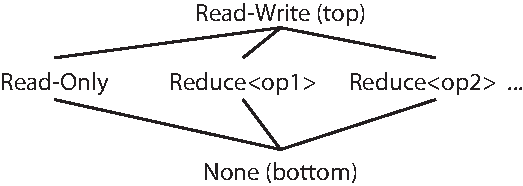
\includegraphics[scale=0.7]{figs/PrivilegeLattice}
\caption{Legion Privileges Semi-Lattice\label{fig:privlattice}}
\end{figure}

The Legion programming model requires that sub-tasks
within a Legion application maintain the following
property: sub-tasks are only permitted to
access fields of logical regions with a subset of the
privileges of their parent task.
We call this property the {\em containment property}.
To be more concrete, in order for the containment 
property to hold for a sub-task, then all of the
following must be true for each logical region
a sub-task requests privileges on:
\begin{itemize}
\item The parent task must also have privileges
      on the specified logical region.
\item For each field, the parent task must also
      have privileges on the specified field.
\item The parent task must have privileges that
      are a (non-strict) superset of the privileges
      requested by the child task as defined by
      the privilege semi-lattice in 
      Figure~\ref{fig:privlattice}.
\end{itemize}
In some ways, the containment property resembles functional
programming models, in which sub-functions only have
access to the data directly passed from their parent
function. The only difference being that Legion 
permits tasks to explicitly side-effect logical regions
in accordance with the declared privileges. The need for
the functional nature of the containment property will
become evident in Section~\ref{subsec:hierarchical} when
we describe the hierarchical scheduling algorithm that
it enables.

As a brief aside, we note that the containment 
property required of Legion programs makes Legion
an interesting hybrid between a functional and 
an imperative programming model. At a coarse-granularity
(between tasks), Legion appears like a functional model
with tasks only accessing subsets of data that their
parent task had access to.  However, at a fine-granularity
tasks are composed of statements that mutate the state
of logical regions, much like imperative programs 
manipulating data in one or more heaps. In many ways,
this approach makes porting code to Legion easier.
Existing imperative code can be wrapped inside of a
task, and only the dependences between tasks based
on region usage need be considered at a functional
level by a Legion implementation.

To this point, we have yet to describe how privileges
are initially created in a Legion program. When a
task creates a logical region it is granted full 
{\tt read-write} privileges for all fields
in the logical region. It is then free to pass
these privileges through sub-task calls to child
tasks.  If the creating task also returns a region
it allocated, the task returns the full
{\tt read-write} privileges to its enclosing parent
task. It is important to note that this happens
automatically and is tracked implicitly by a 
Legion implementation. The implicit nature of
privilege tracking is important because it 
guarantees that privileges cannot be stored 
anywhere in memory or passed to other sub-tasks in any way
except via sub-task calls and tasks completing.
This aspect of privileges will be a crucial element 
in enabling the implementation of the hierarchical 
scheduling algorithm described in 
Section~\ref{subsec:hierarchical} because it implies
privileges are not first-class objects, and can 
therefore always be tracked by a Legion implementation.

In our circuit simulation, each {\tt simulate\_circuit}
task initially holds read-write privileges on both of
the  logical regions that contain all of the node 
and wire data for the circuit graph. Therefore, each
of the sub-tasks launched by {\tt simulate\_circuit}
for the main time-step loop meet the functional property
required by the Legion programming model because all
tasks are asking for a sub-set of privileges that the
parent task holds.

\subsection{Execution Model}
\label{subsec:execmodel}
Before proceeding with our discussion of
the remaining features associated with tasks,
we briefly introduce the Legion execution
model. In Legion, all sub-tasks (and other
operations discussed in Section~\ref{sec:ops})
are launched asynchronously. It is the 
responsibility of the Legion runtime to 
maintain sequential program order semantics
for these sub-tasks and operations. To achieve
high performance, Legion employs implicit
parallelism to discover where sub-tasks and
operations can be run in parallel based on
the logical regions used by sub-tasks and
other operations. Legion allows sub-tasks
and operations to execute in parallel
when they are {\em non-interfering} on 
their logical region arguments. We give
a formal definition of what it means for tasks
and other operations to be non-interfering in 
Section~\ref{sec:noninterference}. One of the 
primary contributions of this thesis is the 
data structures and algorithms for implicitly 
discovering  parallelism based on non-interference.
We cover these techniques in more detail
in Chapters~\ref{chapter:logical} and
\ref{chapter:physical}.

Ensuring that all Legion sub-tasks and other
operations are asynchronous is a key component
of the Legion design. By guaranteeing that Legion
is fully asynchronous, Legion applications can
launch many outstanding sub-tasks and other
operations, allowing a Legion implementation to
automatically discover as much parallelism as
possible. Discovering large amounts of independent
work is crucial to hiding the large latencies
present in modern supercomputers. Finding significant
parallel work also allows a Legion implementation
to hide much of the latency associated with its 
dynamic analyses. To the best of our knowledge,
this fully asynchronous execution model has
no name in the academic literature. We refer
to it as {\em deferred execution}.

The essence of a deferred execution model is
the promise that all operations are asynchronous
and it is the responsibility of the Legion
implementation to maintain the sequential program
order semantics of an application. In order to
avoid exposing latencies, applications should
refrain from performing blocking operations that
might impede a Legion implementation from discovering
additional parallelism. As we will see later in this
section, there are several ways that tasks can block 
their execution. While it is encouraged for tasks to 
run arbitrarily far into the future to expose many 
sub-tasks and operations, there is naturally a limit 
to the number of operations that should be in flight 
from the execution of a given task.  We discuss some 
of the features that Legion employs for limiting the 
number of sub-tasks and operations in flight in 
Sections~\ref{subsec:pipeline}
and \ref{sec:mapbasic}.

Our circuit simulation exemplifies
the benefits that can be obtained from deferred
execution. Since all task launch operations are 
performed asynchronously, the execution of the
the loops on lines 32-36 of Listing~\ref{lst:code_ex}
can be unrolled arbitrarily far, allowing the Legion 
runtime to see a large window of potential tasks to 
run. As we will see in later chapters, the deferred 
execution model will allow a Legion implementation 
to pipeline many of the operations associated with
executing a task and thereby hide the latency both
of dynamic program analysis and communication 
between nodes.

\subsection{Index Space Tasks}
\label{subsec:indextasks}
While the standard way of launching sub-tasks from
a parent task is to launch a single task, Legion
also provides a mechanism for launching many sub-tasks
simultaneously. Legion permits applications 
to issue {\em index space task launches} where many
tasks are launched with a single call. Index space
task launches are useful because they allow for many
tasks to be put in flight simultaneously, which can
help in reducing runtime overheads when many 
child tasks need to be launched. Furthermore,
index space task launches allow applications to 
express important properties about groups of 
tasks including the requirement that they all
be capable of synchronizing with each other 
throughout their execution (see
Chapter~\ref{chapter:relaxed} for more details).
When an index space task launch is performed,
the application specifies an index space of 
points with the understanding that Legion
will create a single task for each point in
the index space. There are numerous index
space task launches in the CG solver shown
in Listing~\ref{lst:cg_ex} (lines 19, 21, 34,
36, 40, 42, 43, 45, 46, and 47). In each case
we launch {\tt num\_pieces} different tasks
for each of the different chunks of the vectors
being computed.

In order to aid applications in describing index
space task launches, Legion supports a special
kind of region requirement called a {\em projection}.
Projection region requirements are different
from normal region requirements in that they
do not need to explicitly name the region
requirements for the task corresponding to 
each point in the index space launch. Instead
projection region requirements allow index
space task launches to name either a logical
region or logical partition to serve as an
upper bound on logical regions on which tasks
within the index space task launch will 
request privileges. In the CG solver in 
Listing~\ref{lst:cg_ex}, all of the index
space task launches use partition projection
requirements with the partitions of the 
vectors and/or sparse matrix as the upper
bound.

Projection region 
requirements also provide a function to be 
invoked by a Legion implementation which takes 
as arguments the upper bound logical region 
or partition and a point in the index 
space launch, and returns the specific logical 
region to be used for the particular task. 
The projection function must be pure, but it 
is provided information about the shape of the logical
region tree that it is traversing in order to
aid its computation. For the most common cases,
Legion provides a built-in projection function 
that linearizes all the points in the index space 
and maps them onto the individual sub-regions of 
a partition modulo the total number of sub-regions.
This built-in function is sufficient for handling
all of the projection requirements in the CG
solver example and is therefore not shown.

Having upper bounds on the 
logical regions that all tasks in an index 
space task launch will access enables a Legion 
implementation to optimize some aspects of dependence 
analysis that we will discuss in 
Chapter~\ref{chapter:logical}.
While index space task launches allow
many tasks to be launched in parallel, 
the Legion programming model does restrict
the regions that individual points access
to be non-interfering with all other
points in the same index space launch.

%To give a concrete example of the utility of index
%space task launches, consider the code for launching
%the different phases of the circuit simulation in
%the main time-step loop in Listing~\ref{lst:code_ex}.
%In the current example, there is a {\tt for} loop 
%that is used to launch a sub-task for each piece
%for every phase (lines 33-35). Alternatively, we
%could have specified a single index space task launch
%for each phase with the index space being a one
%dimensional array equal to the number of pieces.
%A separate sub-task would then be created for handling
%each piece in the index space task launch for a given
%phase. For each index space task launch we would use
%projection region requirements that named the 
%{\tt p\_pvt\_nodes}, {\tt p\_shr\_nodes}, {\tt p\_ghost\_nodes},
%and {\tt p\_wires} partitions as upper bounds for 
%the privileges. A simple projection function would 
%then pick the correct logical region for each point
%task by taking the task's point ID as a the number
%for the circuit piece to handle. In practice, our
%actual implementation of the circuit simulation
%uses index space task launches to achieve high 
%performance.

\subsection{Futures}
\label{subsec:futures}
Much like traditional functions, Legion tasks
are permitted to return values. When a
task call is performed in Legion it does
not block. This is an essential component
of the Legion deferred execution model. The 
asynchronous nature of tasks in Legion necessitates 
that a place-holder object be used to represent the
return values from a task. As is common in the
literature, we refer to these values as {\em futures}.

In the case of index space task launches,
a {\em future map} can be returned which 
contains a single future entry for each point
in the index space of tasks launched. Applications
can then extract these futures and use them
as if they had been generated by a single task
launch. Alternatively, in some cases, applications
might want to reduce all the futures from an 
index space task launch down to a single value.
For example, consider the dot-product computations
done by the CG solver in Listing~\ref{lst:cg_ex}
(line 34). Each task in the dot-product index
space task launch computes a sum for a different
part of the vectors. All of these values need to 
be reduced down to a single value for the dot product,
therefore a sum reduction (indicated by {\tt <+>} on the
index space launch) is passed as the reduction function to 
use for  combining the results of an index space
tasks' return values into a single future value.

Future values can be used in one of three
different ways. First, a parent task that
has a future value for one of its child tasks
can explicitly wait on the future result. This
blocks the parent task until the future is 
{\em complete} (when the child task completes
and returns the value). Waiting on a future
should in general be an uncommon operation in
Legion as it prevents the parent task from
continuing execution and exposing additional
work to the Legion runtime.
Waiting on a future result also has ramifications
for resilience which we discuss in 
Chapter~\ref{chapter:resilience}. Futures are not 
first-class objects and are not permitted to be 
stored in logical regions. Applications must 
explicitly wait on a future result
to write the value into memory.

The second way that a future can be used is that
it can be passed as a input parameter to another
child task in the same parent task. Passing a future
as an argument to another sub-task launch does
not cause the additional sub-task launch to
block. As an example, notice the {\tt divide}
function in the CG solver on lines 38 and 44. This
task takes two futures and uses their values to 
compute a new future that is the result of dividing
the first future by the second. This way of using 
futures is much more consistent with Legion's 
deferred execution model because it avoids
blocking the parent task. 

The third way to use a future value is to create
a predicate value from it. Boolean futures can
automatically be converted into predicates,
while other future types can be turned into
predicates with an associated function that
evaluates the value of the future and 
returns a boolean. Line 47 of the CG solver
creates a predicate from a boolean future
value returned by the {\tt test\_convergence}
task. As we will see in the next section,
these predicates can be used for predicating
task execution.

%To give a concrete example of how futures might be
%used, consider a modified version of our circuit
%simulation without a driving power supply. Under
%these conditions, a time-step loop is unnecessary.
%Instead we would want to iterate until the 
%circuit reaches a steady state. Testing for a 
%steady state requires detecting if all of the 
%pieces have stopped changing. To handle this case
%we would likely modify the {\tt update\_voltages}
%task to return a boolean indicating whether
%a convergence criteria had been met. By merging
%these boolean  futures of all the pieces together 
%we could determine if the entire circuit had 
%reached a steady state.

\subsection{Predicated Execution}
\label{subsec:speculation}
One of the more important features of Legion
is its ability to allow sub-task launches
to be predicated. Predicated sub-tasks allow
parent tasks to continue executing and
launching sub-tasks without needing to
block to resolve conditional values
(e.g. for {\tt if} statements or loops).
For example, consider the CG solver in
Listing~\ref{lst:cg_ex}. We
start out with a {\tt loop\_pred} predicate
that is used to predicate all task launches
in the iterative loop which we indicate by 
the syntax {\tt @loop\_pred} in any task
launch. The predicate starts out as {\tt true}
and then is converted from a future value 
that is returned by the {\tt test\_convergence}
task (line 47) at the end of every iteration.
In this way, the CG solver unrolls the loop and
issues tasks even without knowing whether
the computation has converged or not. This permits the runtime
to begin the analysis for these tasks even before
it knows if they will ultimately be executed.
In an optimized version of the CG solver, we use
a tunable variable to control how far ahead we
want to unroll the loop. We further discuss the 
need for predicates in Section~\ref{subsec:speculation}.

%For example, in our modified circuit simulation
%that iterates until reaching a steady state, 
%the simulation would need to continue
%executing until it converged. Doing so requires
%testing a convergence condition that could block
%a parent task until the result was known. This
%would significantly hinder 
%Legion's deferred execution model. Instead,
%using predicates, task launches for the next time
%step can be predicated based on a predicate 
%constructed from the merged futures described in 
%Section~\ref{subsec:futures}.
%Predicates therefore add a very natural
%way for dealing with conditionals in a
%deferred execution model.

A separate issue involving predication is
whether or not a Legion implementation is permitted 
to speculate on the values of predicates in
order to start executing predicated tasks
before the predicate value is known. In keeping
with our second design principle, the
decision of when and where to speculate is
independent of the specification of the 
algorithm for an application and 
it is therefore determined by Legion
mapper objects. We discuss how speculation
can be directed by a Legion mapper in
Section~\ref{subsec:specexec}.

\subsection{Task Variants}
\label{subsec:variants}
Determining the correct algorithm to use for
different applications is not always an 
obvious decision, especially in the context
of different target architectures. Legion
therefore allows applications to register
multiple functionally equivalent {\em variants}
of the same task. This idea is borrowed
from Sequoia~\cite{Sequoia06}. By specifying
multiple functionally equivalent variants
for the same task, Legion allows applications
to explore different algorithms as part of
the process of mapping an application to 
a target architecture. We discuss how 
Legion mappers can select which variant of 
a task to use in Section~\ref{subsec:maptask}.

Another important property of Legion task variants
is that they can be used to specialize both task
implementations as well as algorithms for a 
particular target architecture. Applications can
explicitly register different task variants for
a target processor kind. Alternatively, the Legion
programming model also permits the registration 
of task {\em generators}. Task generators are
meta-functions capable of generating specialized
variants given constraints on the kind of processor
and the layout of the physical instances for the
task. We cover task generators in greater detail
in Section~\ref{subsec:generators}.

\subsection{Task Qualifiers}
\label{subsec:qualifiers}
The final aspect of Legion tasks is the
ability for applications to add qualifiers on
task variants. Task qualifiers provide additional
information to the Legion runtime regarding 
operations that task will (or will not) do at
runtime that can aid in performance optimizations.
There are three different kinds of qualifiers that 
can be associated with a task: {\em leaf}, 
{\em inner}, and {\em idempotent}. We cover
each qualifier in turn. Note that tasks are
not required to specify any of these qualifiers,
as the qualifiers only provide opportunities
for performance optimizations for a Legion
implementation.

The first qualifier that can be associated with
a task variant is whether the task variant
is a {\em leaf} task. A leaf task is a task 
variant that is only permitted to operate on 
the region data that it requested, and not to 
perform any Legion operations. Since it performs 
no Legion operations, it is not permitted to 
launch any sub-tasks and is therefore always a 
leaf in the dynamic task tree. 
Leaf tasks allow a Legion implementation
to reduce the meta-data associated with a task.

The second qualifier that can be associated with
a task variant is whether the task variant is
an {\em inner} task. An inner task is the opposite
of a leaf task. Inner tasks are not permitted to
actually access the logical regions they requested
privileges on, but are only allowed to launch
sub-tasks and pass privileges through to child
tasks. Inner tasks can perform any arbitrary
Legion operations that are necessary as long
as they do not access logical region data. Inner
tasks allow a Legion implementation to begin
executing a task even before its logical region
data is ready in order to discover additional task
parallelism generated by the inner task.

The final qualifier that can be specified for
a task variant is whether the task variant
is {\em idempotent}. A task is idempotent if
the only side-effects that it performs are
modifications to logical regions. If the task
performs alternative side effects (e.g.
writing files, printing output, etc.) then 
it cannot be considered
idempotent. In general the majority of tasks
in a Legion application should be idempotent
with only a few tasks accessing external 
resources. Idempotent tasks enable 
resiliency optimizations that are discussed
in more detail in Chapter~\ref{sec:resilience}.

In our circuit simulation from Section~\ref{sec:circuit},
all of the sub-tasks launched for calculating
currents, distributing charge, and updating voltages
could be annotated as leaf tasks because they
do not launch any sub-tasks. These tasks could also
be labeled as idempotent because they only mutate
the logical regions for which they have requested
privileges. The {\tt simulate\_circuit} task is a
different; depending on whether it reads and/or
writes information about the circuit to/from a 
file determines whether it is idempotent or not.

\section{Physical Instances}
\label{sec:phyinst}
While logical regions provide names for describing
different sets of program data, the execution of
tasks requires access to actual data in a specific
place. {\em Physical regions} describe an actual
instance of a logical region that resides in 
a specific memory in the memory hierarchy and 
represents a specific layout of the data contained
within the logical region. The Legion programming
model guarantees that when a task starts it will
have physical regions for each of the region 
requirements that it requested. The choice of
where these physical regions are located and how
they are laid out in memory is determined by
Legion mapper objects discussed in 
Chapter~\ref{chapter:mapping}, but Legion mappers
are only permitted to map physical instances into
memories that are visible from the target
processor for a task.

\subsection{Logical to Physical Mapping}
\label{subsec:logtophys}
The distinction between logical and physical regions
is unfamiliar to programmers new to Legion, but there
is a simple analogy to conventional languages.
In most modern programming languages, compilers
automatically manage the mapping from variables
to physical registers used in machine assembly
code. Logical and physical regions are analogous
to variables and registers. Currently, 
it is the responsibility of the Legion application
developer to manage both logical and physical
regions in the same application\footnote{We note that as of
the time of the publication of this thesis, a Legion
language is in development that does not require
a distinction between logical and physical regions.
Instead the Legion language compiler can automatically
manage the logical and physical regions of the Legion
programming model automatically, much in the same
way that modern compilers manage the mapping from 
variables to hardware registers.}.

One important detail regarding physical regions is
that they must be {\em unmapped} before launching
sub-tasks that use the corresponding logical region
that the physical region represents. Unmapping a 
physical region before launching a sub-task that uses
the same logical region is necessary to avoid data 
races and consistency problems between a parent task 
and a child task accessing the same data. In practice, 
failure to unmap regions used by child tasks can result 
in a deadlock where a child task depends on its parent
task and the parent task cannot complete until the
child task completes. To maintain the
correctness of a Legion application, a Legion
implementation should detect when a sub-task is
accessing a logical region mapped by the parent
and issue the corresponding unmap and re-map
operations immediately before and after the 
sub-task launch. Applications can optimize
performance by unmapping physical regions and
then re-mapping them only when they need to
be accessed. We discuss how mapping and unmapping
operations are performed in Section~\ref{sec:ops}. 

\subsection{Accessors}
\label{subsec:accessors}
To maintain one of the Legion core design principles
a necessary level of indirection is required to
access data from physical regions. Physical regions
are located in a specific memory in the memory 
hierarchy and have a given layout.  Both of these
properties of a physical region are determined by
the mapping process. To maintain the invariant that
a Legion application is machine-independent,
we require data from physical regions
to be accessed using {\em accessor} objects. Accessors
abstract the details of physical region locations
and data layouts when performing reads, writes, and
reductions to a physical instance. In many cases,
accessors can be specialized at runtime based on
physical region properties, but Legion also provides
general accessors capable of accessing any physical
region.

In addition to accessors, Legion task variants
can also be specified with generators that do not
require accessors. Using meta-programming techniques
generators can emit specialized code for specific
physical regions at runtime without requiring 
general and specialized accessor objects for different
physical regions. We discuss generators in more 
detail in Section~\ref{subsec:generators}.


\section{Operations: Mapping, Copies, and Barriers}
\label{sec:ops}
In addition to allowing parent tasks to launch 
sub-tasks, the Legion programming model also allows
parent tasks to issue other kinds of operations.
Some of these operations function primarily as 
productivity features, while others are also 
useful for achieving high performance. For example,
inline mapping operations are mainly a productivity
operation because they allow applications to 
immediately gain access to a physical instance of
a logical region after the region has been created.
Alternatively, explicit region-to-region copies
are valuable for performance as they allow 
applications to explicitly describe data movement
between regions while allowing the runtime to
optimize the implementation of these data transfers.

In keeping with Legion's deferred execution model
all of these operations are issued asynchronously.
It is the responsibility of a Legion implementation to
properly order these operations with respect to
other operations in the stream of sub-operations.
A Legion runtime will automatically infer dependences
between operations based on region requirements.

\subsection{Inline Mappings}
\label{subsec:inline}
A natural operation that Legion
supports (and one that was omitted from earlier
Legion versions), is {\em inline mappings}. In
older versions of Legion, the only way to 
map a physical instance of a logical region was
to launch a sub-task that would map the logical
region as part of the task being mapped. However,
in many cases, it is useful for tasks to decide 
to map a logical region locally as part of their
execution. For example, it would be natural for
the {\tt simulate\_circuit} task from our circuit
simulation to perform an inline mapping
when loading a circuit topology from a file.
To handle mapping and unmapping of logical regions
within a task, inline mapping and unmapping 
operations are performed.

An inline mapping operation takes a region requirement
similar to sub-task launches, but instead returns
a handle to a physical region that will 
correspond to a mapped physical instance once the
operation completes. In many ways the physical region 
handle acts like a future. Before an 
application can create an accessor to the physical 
instance it must explicitly wait for the region to be ready.
We note that needing to explicitly wait on the physical
region to be ready runs counter to
deferred execution, but there is no 
alternative when the data in a logical region must
be explicitly accessed by a task. To encourage
the discovery of as much parallelism as possible,
we make inline mapping launches asynchronous, thereby
allowing applications to perform as much additional
work as possible before it becomes necessary to wait 
for a physical region to be ready.

In addition to inline mappings, Legion also allows
applications to launch unmap operations for 
physical regions. Unmapping operations enable 
tasks to indicate that they are no longer accessing
a physical region, allowing other operations
such as sub-tasks to avoid dependences on the
parent task. Unmap operations can be used to
unmap physical regions that were mapped either
directly by the parent task or by inline
mapping operations. Once a physical region
has been unmapped, it can always be remapped
using an inline mapping operation.

\subsection{Explicit Region Copies}
\label{subsec:copies}
Another operation that has been useful for
developing Legion applications is the
ability to issue explicit copies between fields
in different logical regions. In general, most
Legion applications allow the Legion runtime to
implicitly issue data movement operations based
on logical region uses.  However, some applications
explicitly manage different logical regions for
the same data. As a simple example, the CG solver
in Listing~\ref{lst:cg_ex} issues an explicit
region-to-region copy operation on line 26 to 
initialize the data in a new logical region.
A more substantial example of the use of explicit
copy operations will be the
S3D application that we introduce in 
Chapter~\ref{chapter:s3d} that maintains explicit
ghost cell logical regions that are updated
using explicit region-to-region copies.

Like other operations, explicit region-to-region
copies are issued using region requirements to
describe the source and destination logical regions
as well as the fields to be copied between them.
Legion requires that the
destination logical region have an index space
that is {\em dominated} by the index space of
the source logical region. An index space $i_0$
dominates and index space $i_1$, if $i_0$ contains
all of the points of $i_1$.
The two index spaces do not need to come from 
the same index space tree, but they do need to
be the same dimension to check for dominance.
Checking for dominance guarantees that a full 
copy of the data will be manifested in the 
destination logical region and ensures that no
values in the destination region are left
undefined by the copy. Similar to both 
sub-tasks and inline mapping operations, the
region requirements for copy operations are 
mapped by a mapper object.

\subsection{Execution Fences}
\label{subsec:fences}
The final kind of operation that Legion supports
are {\em execution fences}. Execution fences
provide a means for applications to delineate
sets of operations and sub-tasks into epochs,
either for the purpose of mapping or execution.
It is important to note that execution fences
are not barriers. Execution fences do not block
execution of a parent task, but instead are
issued asynchronously like all other operations
into the stream of operations and sub-tasks.

The Legion programming model supports two kinds
of execution fences: {\em mapping} fences and
{\em execute} fences. Mapping fences require
that all operations prior to the fence have 
completed mapping before any operations after
the mapping fence are permitted to begin mapping.
In Chapter~\ref{chapter:logical} we will see
two examples of how mapping fences can be 
used for optimizations. Mapping fences are
also useful for providing context information to mapper 
objects by creating different epochs of a parent 
task's execution (e.g. operations and sub-tasks
corresponding to specific time-steps).

Alternatively, execute fences ensure that all
sub-operations in a parent task have finished
executing before any operations after the fence
are permitted to execute. Execute fences provide
a mechanism for adding additional constraints
on the execution order of operations (in addition
to logical region data dependences and future
dependences). Execute fences are a very blunt
tool and should only be used at a coarse
granularity for controlling execution.


\section{Machine Independent Specification}
\label{sec:indepspec}
Throughout this chapter we have introduced many 
features of the Legion programming model. In the
process we have highlighted important decisions
made in the design that reflect our initial design
principles laid out in Section~\ref{sec:design}.
The absence of certain features is equally important.
Our entire discussion 
of the Legion programming model has avoided 
describing where tasks are scheduled or where
logical regions representing program data are
placed in the memory hierarchy. In cases where
variables depended on the target machine, we
allow users to directly declare these variables
as tunables and defer assigning values until
the mapper chooses a value at runtime. Consequently,
all aspects of a Legion program that may depend
on the target architecture are explicitly decoupled
from the Legion program. It is important to note
that the only reason that this is possible is 
because Legion provides abstractions for both
computation (tasks) and data (logical regions).
While many other programming systems have abstractions
for parallel computation, the novel aspect of 
Legion is the introduction of logical regions as
the basis for an abstract data model. With logical
regions, all aspects of a program specification can
be completely decoupled from its mapping.

